\documentclass[twoside]{book}

% Packages required by doxygen
\usepackage{fixltx2e}
\usepackage{calc}
\usepackage{doxygen}
\usepackage[export]{adjustbox} % also loads graphicx
\usepackage{graphicx}
\usepackage[utf8]{inputenc}
\usepackage{makeidx}
\usepackage{multicol}
\usepackage{multirow}
\PassOptionsToPackage{warn}{textcomp}
\usepackage{textcomp}
\usepackage[nointegrals]{wasysym}
\usepackage[table]{xcolor}

% Font selection
\usepackage[T1]{fontenc}
\usepackage[scaled=.90]{helvet}
\usepackage{courier}
\usepackage{amssymb}
\usepackage{sectsty}
\renewcommand{\familydefault}{\sfdefault}
\allsectionsfont{%
  \fontseries{bc}\selectfont%
  \color{darkgray}%
}
\renewcommand{\DoxyLabelFont}{%
  \fontseries{bc}\selectfont%
  \color{darkgray}%
}
\newcommand{\+}{\discretionary{\mbox{\scriptsize$\hookleftarrow$}}{}{}}

% Page & text layout
\usepackage{geometry}
\geometry{%
  a4paper,%
  top=2.5cm,%
  bottom=2.5cm,%
  left=2.5cm,%
  right=2.5cm%
}
\tolerance=750
\hfuzz=15pt
\hbadness=750
\setlength{\emergencystretch}{15pt}
\setlength{\parindent}{0cm}
\setlength{\parskip}{3ex plus 2ex minus 2ex}
\makeatletter
\renewcommand{\paragraph}{%
  \@startsection{paragraph}{4}{0ex}{-1.0ex}{1.0ex}{%
    \normalfont\normalsize\bfseries\SS@parafont%
  }%
}
\renewcommand{\subparagraph}{%
  \@startsection{subparagraph}{5}{0ex}{-1.0ex}{1.0ex}{%
    \normalfont\normalsize\bfseries\SS@subparafont%
  }%
}
\makeatother

% Headers & footers
\usepackage{fancyhdr}
\pagestyle{fancyplain}
\fancyhead[LE]{\fancyplain{}{\bfseries\thepage}}
\fancyhead[CE]{\fancyplain{}{}}
\fancyhead[RE]{\fancyplain{}{\bfseries\leftmark}}
\fancyhead[LO]{\fancyplain{}{\bfseries\rightmark}}
\fancyhead[CO]{\fancyplain{}{}}
\fancyhead[RO]{\fancyplain{}{\bfseries\thepage}}
\fancyfoot[LE]{\fancyplain{}{}}
\fancyfoot[CE]{\fancyplain{}{}}
\fancyfoot[RE]{\fancyplain{}{\bfseries\scriptsize Generated by Doxygen }}
\fancyfoot[LO]{\fancyplain{}{\bfseries\scriptsize Generated by Doxygen }}
\fancyfoot[CO]{\fancyplain{}{}}
\fancyfoot[RO]{\fancyplain{}{}}
\renewcommand{\footrulewidth}{0.4pt}
\renewcommand{\chaptermark}[1]{%
  \markboth{#1}{}%
}
\renewcommand{\sectionmark}[1]{%
  \markright{\thesection\ #1}%
}

% Indices & bibliography
\usepackage{natbib}
\usepackage[titles]{tocloft}
\setcounter{tocdepth}{3}
\setcounter{secnumdepth}{5}
\makeindex

% Hyperlinks (required, but should be loaded last)
\usepackage{ifpdf}
\ifpdf
  \usepackage[pdftex,pagebackref=true]{hyperref}
\else
  \usepackage[ps2pdf,pagebackref=true]{hyperref}
\fi
\hypersetup{%
  colorlinks=true,%
  linkcolor=blue,%
  citecolor=blue,%
  unicode%
}

% Custom commands
\newcommand{\clearemptydoublepage}{%
  \newpage{\pagestyle{empty}\cleardoublepage}%
}

\usepackage{caption}
\captionsetup{labelsep=space,justification=centering,font={bf},singlelinecheck=off,skip=4pt,position=top}

%===== C O N T E N T S =====

\begin{document}

% Titlepage & ToC
\hypersetup{pageanchor=false,
             bookmarksnumbered=true,
             pdfencoding=unicode
            }
\pagenumbering{roman}
\begin{titlepage}
\vspace*{7cm}
\begin{center}%
{\Large linux-\/list }\\
\vspace*{1cm}
{\large Generated by Doxygen 1.8.11}\\
\end{center}
\end{titlepage}
\clearemptydoublepage
\tableofcontents
\clearemptydoublepage
\pagenumbering{arabic}
\hypersetup{pageanchor=true}

%--- Begin generated contents ---
\chapter{Data Structure Index}
\section{Data Structures}
Here are the data structures with brief descriptions\+:\begin{DoxyCompactList}
\item\contentsline{section}{\hyperlink{structkool__list}{kool\+\_\+list} }{\pageref{structkool__list}}{}
\item\contentsline{section}{\hyperlink{structlist__head}{list\+\_\+head} }{\pageref{structlist__head}}{}
\item\contentsline{section}{\hyperlink{structlistitem}{listitem} }{\pageref{structlistitem}}{}
\item\contentsline{section}{\hyperlink{structteststruct}{teststruct} }{\pageref{structteststruct}}{}
\end{DoxyCompactList}

\chapter{Data Structure Documentation}
\hypertarget{structkool__list}{}\section{kool\+\_\+list Struct Reference}
\label{structkool__list}\index{kool\+\_\+list@{kool\+\_\+list}}


Collaboration diagram for kool\+\_\+list\+:
\nopagebreak
\begin{figure}[H]
\begin{center}
\leavevmode
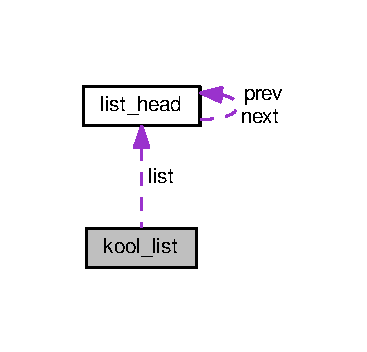
\includegraphics[width=176pt]{structkool__list__coll__graph}
\end{center}
\end{figure}
\subsection*{Data Fields}
\begin{DoxyCompactItemize}
\item 
int {\bfseries to}\hypertarget{structkool__list_ac0ed249f3db34b8135fd2717bda56844}{}\label{structkool__list_ac0ed249f3db34b8135fd2717bda56844}

\item 
struct \hyperlink{structlist__head}{list\+\_\+head} {\bfseries list}\hypertarget{structkool__list_a1f00f18b91d5a820f2c43064243aa86e}{}\label{structkool__list_a1f00f18b91d5a820f2c43064243aa86e}

\item 
int {\bfseries from}\hypertarget{structkool__list_a16d981023742d3bd53f1385790714190}{}\label{structkool__list_a16d981023742d3bd53f1385790714190}

\end{DoxyCompactItemize}


The documentation for this struct was generated from the following file\+:\begin{DoxyCompactItemize}
\item 
tests/test\+\_\+list.\+c\end{DoxyCompactItemize}

\hypertarget{structlist__head}{}\section{list\+\_\+head Struct Reference}
\label{structlist__head}\index{list\+\_\+head@{list\+\_\+head}}


{\ttfamily \#include $<$list.\+h$>$}



Collaboration diagram for list\+\_\+head\+:
\nopagebreak
\begin{figure}[H]
\begin{center}
\leavevmode
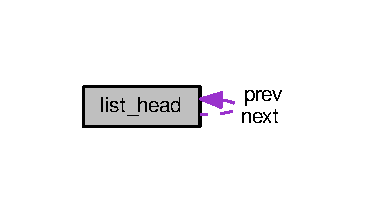
\includegraphics[width=176pt]{structlist__head__coll__graph}
\end{center}
\end{figure}
\subsection*{Data Fields}
\begin{DoxyCompactItemize}
\item 
struct \hyperlink{structlist__head}{list\+\_\+head} $\ast$ {\bfseries prev}\hypertarget{structlist__head_ad8f06cb209b17c3a4a5b24cad8793f72}{}\label{structlist__head_ad8f06cb209b17c3a4a5b24cad8793f72}

\item 
struct \hyperlink{structlist__head}{list\+\_\+head} $\ast$ {\bfseries next}\hypertarget{structlist__head_afb6f2172d12efd37f00bb623a6885f2a}{}\label{structlist__head_afb6f2172d12efd37f00bb623a6885f2a}

\end{DoxyCompactItemize}


\subsection{Detailed Description}
struct \hyperlink{structlist__head}{list\+\_\+head} -\/ Head and node of a double-\/linked list \+: pointer to the previous node in the list \+: pointer to the next node in the list

The simple double-\/linked list consists of a head and nodes attached to this head. Both node and head share the same struct type. The list\+\_\+$\ast$ functions and macros can be used to access and modify this data structure.

The  pointer of the list head points to the last list node of the list and  points to the first list node of the list. For an empty list, both member variables point to the head.

The list nodes are usually embedded in a container structure which holds the actual data. Such an container object is called entry. The helper list\+\_\+entry can be used to calculate the object address from the address of the node. 

The documentation for this struct was generated from the following files\+:\begin{DoxyCompactItemize}
\item 
include/list.\+h\item 
include/mylist.\+h\end{DoxyCompactItemize}

\hypertarget{structlistitem}{}\section{listitem Struct Reference}
\label{structlistitem}\index{listitem@{listitem}}


Collaboration diagram for listitem\+:
\nopagebreak
\begin{figure}[H]
\begin{center}
\leavevmode
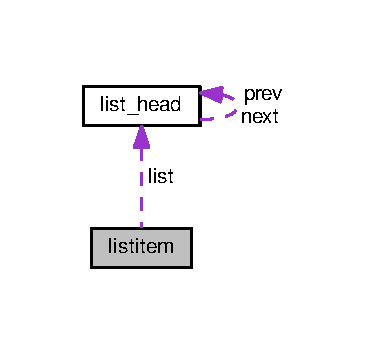
\includegraphics[width=176pt]{structlistitem__coll__graph}
\end{center}
\end{figure}
\subsection*{Data Fields}
\begin{DoxyCompactItemize}
\item 
uint16\+\_\+t {\bfseries i}\hypertarget{structlistitem_a78f7a37dba921e0b0347b960fb40bc51}{}\label{structlistitem_a78f7a37dba921e0b0347b960fb40bc51}

\item 
struct \hyperlink{structlist__head}{list\+\_\+head} {\bfseries list}\hypertarget{structlistitem_a1f00f18b91d5a820f2c43064243aa86e}{}\label{structlistitem_a1f00f18b91d5a820f2c43064243aa86e}

\end{DoxyCompactItemize}


The documentation for this struct was generated from the following file\+:\begin{DoxyCompactItemize}
\item 
private/common.\+h\end{DoxyCompactItemize}

\hypertarget{structteststruct}{}\section{teststruct Struct Reference}
\label{structteststruct}\index{teststruct@{teststruct}}
\subsection*{Data Fields}
\begin{DoxyCompactItemize}
\item 
int {\bfseries a}\hypertarget{structteststruct_aa4c2a5552e9bc49b1816ff532f558c74}{}\label{structteststruct_aa4c2a5552e9bc49b1816ff532f558c74}

\item 
int {\bfseries b}\hypertarget{structteststruct_a148e3876077787926724625411d6e7a9}{}\label{structteststruct_a148e3876077787926724625411d6e7a9}

\end{DoxyCompactItemize}


The documentation for this struct was generated from the following file\+:\begin{DoxyCompactItemize}
\item 
tests/containerof.\+c\end{DoxyCompactItemize}

%--- End generated contents ---

% Index
\backmatter
\newpage
\phantomsection
\clearemptydoublepage
\addcontentsline{toc}{chapter}{Index}
\printindex

\end{document}
